

\newcommand{\doi}[1]{\def\@doi{#1}}
\documentclass[9pt,twocolumn,twoside,notitlepage]{article}
\usepackage{algorithm}
\usepackage{graphicx,xcolor}
\usepackage{minted}
\usepackage{authblk}
\usepackage{amsmath,esint}
\usepackage[colorlinks]{hyperref}
\usepackage{abstract}
\renewcommand{\abstractname}{}    % clear the title
\renewcommand{\absnamepos}{empty} % originally center
\title{UW Toroidal Shell: Moment of Inertia about z axis }
\author[1,2,3]{\normalfont\sffamily\bfseries\scshape\fontsize{12}{14}\selectfont \textcolor{olive} {PlaidML EDSL implementation}}
\begin{document}

\twocolumn[
  \begin{@twocolumnfalse}
    \maketitle
 \begin{abstract}
Moment of inertia about z axis computed for torodial shell with major radius 1 and minor radius 0.1.

\end{abstract}
  \end{@twocolumnfalse}
  ]


\textbf{Problem: } 
$$\iint_S  x^2 + y^2 \,dS$$
where S is defined by :\newline $f(x,y,z)=\sqrt{x^2+y^2}-1)^2+z^2 - 0.1^2=0$
 \begin{figure}[htbp]
 \centering
 \fbox{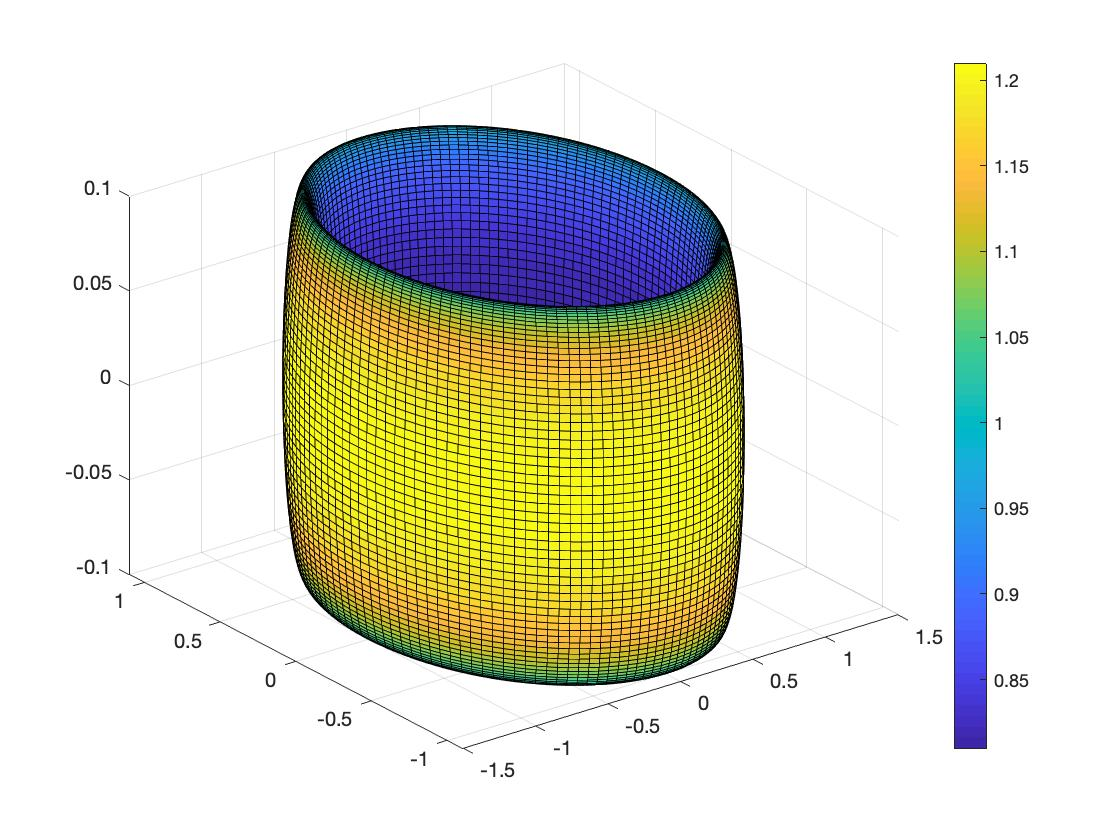
\includegraphics[width=.8\linewidth]{Toroidal_shell_moment.jpg}}
 \caption{Toroidal shell, $R= 1$, $r=0.1$, Color represents $g(x,y,z)=x^2+y^2$}
 \end{figure}

\textbf{Solution steps:}\newline
1. create a grid of points in the x,y,z plane \newline
2. compute $f$ and $g$ on all points on the grid\newline
3. compute $\sqrt{\nabla f \cdot \nabla f}$\newline
4. compute $\nabla g \cdot \nabla \chi (f)$\newline
5. compute $\rho = -1 * g * \frac{\nabla g \cdot \nabla 
\chi}{\sqrt{\nabla f \cdot \nabla f}}$ \newline
6. compute $(\sum \rho)*\delta^3$

%\section{EDSL Sample Code}
\begin{algorithm}
\caption{EDSL Sample Code}\label{euclid}
\inputminted{python}{partial_diff.py}
\hyperlink{https://github.com/plaidml/plaidml/tree/master/networks/scitile}{https://github.com/plaidml/plaidml/tree/master/networks/scitile}
\end{algorithm}

%\subsection{Performance}
%Initial performance numbers are listed below: 
\begin{table}[htbp]
\centering
%\caption{\bf Shape Functions for Quadratic Line Elements}
\begin{tabular}{ccc}
\hline
backend & device & runtime \\
\hline
CUDA  & GeForce GTX 1070  & 0.0069 \\
plaidml2 + opencl & GeForce GTX 1070 & 0.0112 \\
plaidml2 + LLVM  & 2.6 GHz Intel Xeon E5-2670 & 0.2774 \\
plaidml2 + LLVM  &  2.6 GHz Intel Core i7 & 0.0933\\
plaidml2 + opencl & AMD FIJI & 0.0413 \\
plaidml2 + opencl & AMD GFX906 & 0.0235\\
plaidml2 + metal & AMD radeon pro 560x & 0.0552 \\
plaidml2 + metal &  Intel UHD graphics 630 & 0.0597 \\
\hline
\end{tabular}
  \label{tab:shapefunctions}
\end{table}

\end{document}
